\section{Experimental results}

\subsection{Epigenomic experiments}

\subsubsection{Promoters}

In this section are reported the experiment results for active vs
inactive promoters task using epigenomic data. For each metric there are
a table and a plot to confront the learning machine performance.
\newpage
\textbf{Accuracy}

\begin{longtable}[]{@{}lll@{}}
\toprule
\textbf{Models} & \textbf{Training} & \textbf{Test}\tabularnewline
\midrule
\endhead
DecisionTree & mean = 0.7241 & mean = 0.7148\tabularnewline
& STD = 0.0124 & STD = 0.0123\tabularnewline
RandomForest & mean = 0.7522 & mean = 0.7408\tabularnewline
& STD = 0.0014 & STD = 0.0022\tabularnewline
Perceptron & mean = 0.883 & mean = 0.882\tabularnewline
& STD = 0.0005 & STD = 0.0015\tabularnewline
MLP & mean = 0.9638 & mean = 0.8621\tabularnewline
& STD = 0.0041 & STD = 0.0057\tabularnewline
FFNN\_1 & mean = 0.956 & mean = 0.8634\tabularnewline
& STD = 0.0023 & STD = 0.0037\tabularnewline
FFNN\_2 & mean = 0.885 & mean = 0.8848\tabularnewline
& STD = 0.0002 & STD = 0.0002\tabularnewline
FFNN\_3 & mean = 0.8895 & mean = 0.8854\tabularnewline
& STD = 0.0038 & STD = 0.0007\tabularnewline
FFNN\_4 & mean = 0.8886 & mean = 0.884\tabularnewline
& STD = 0.0007 & STD = 0.0011\tabularnewline
\bottomrule
\end{longtable}

\begin{figure}[h!]
\centering
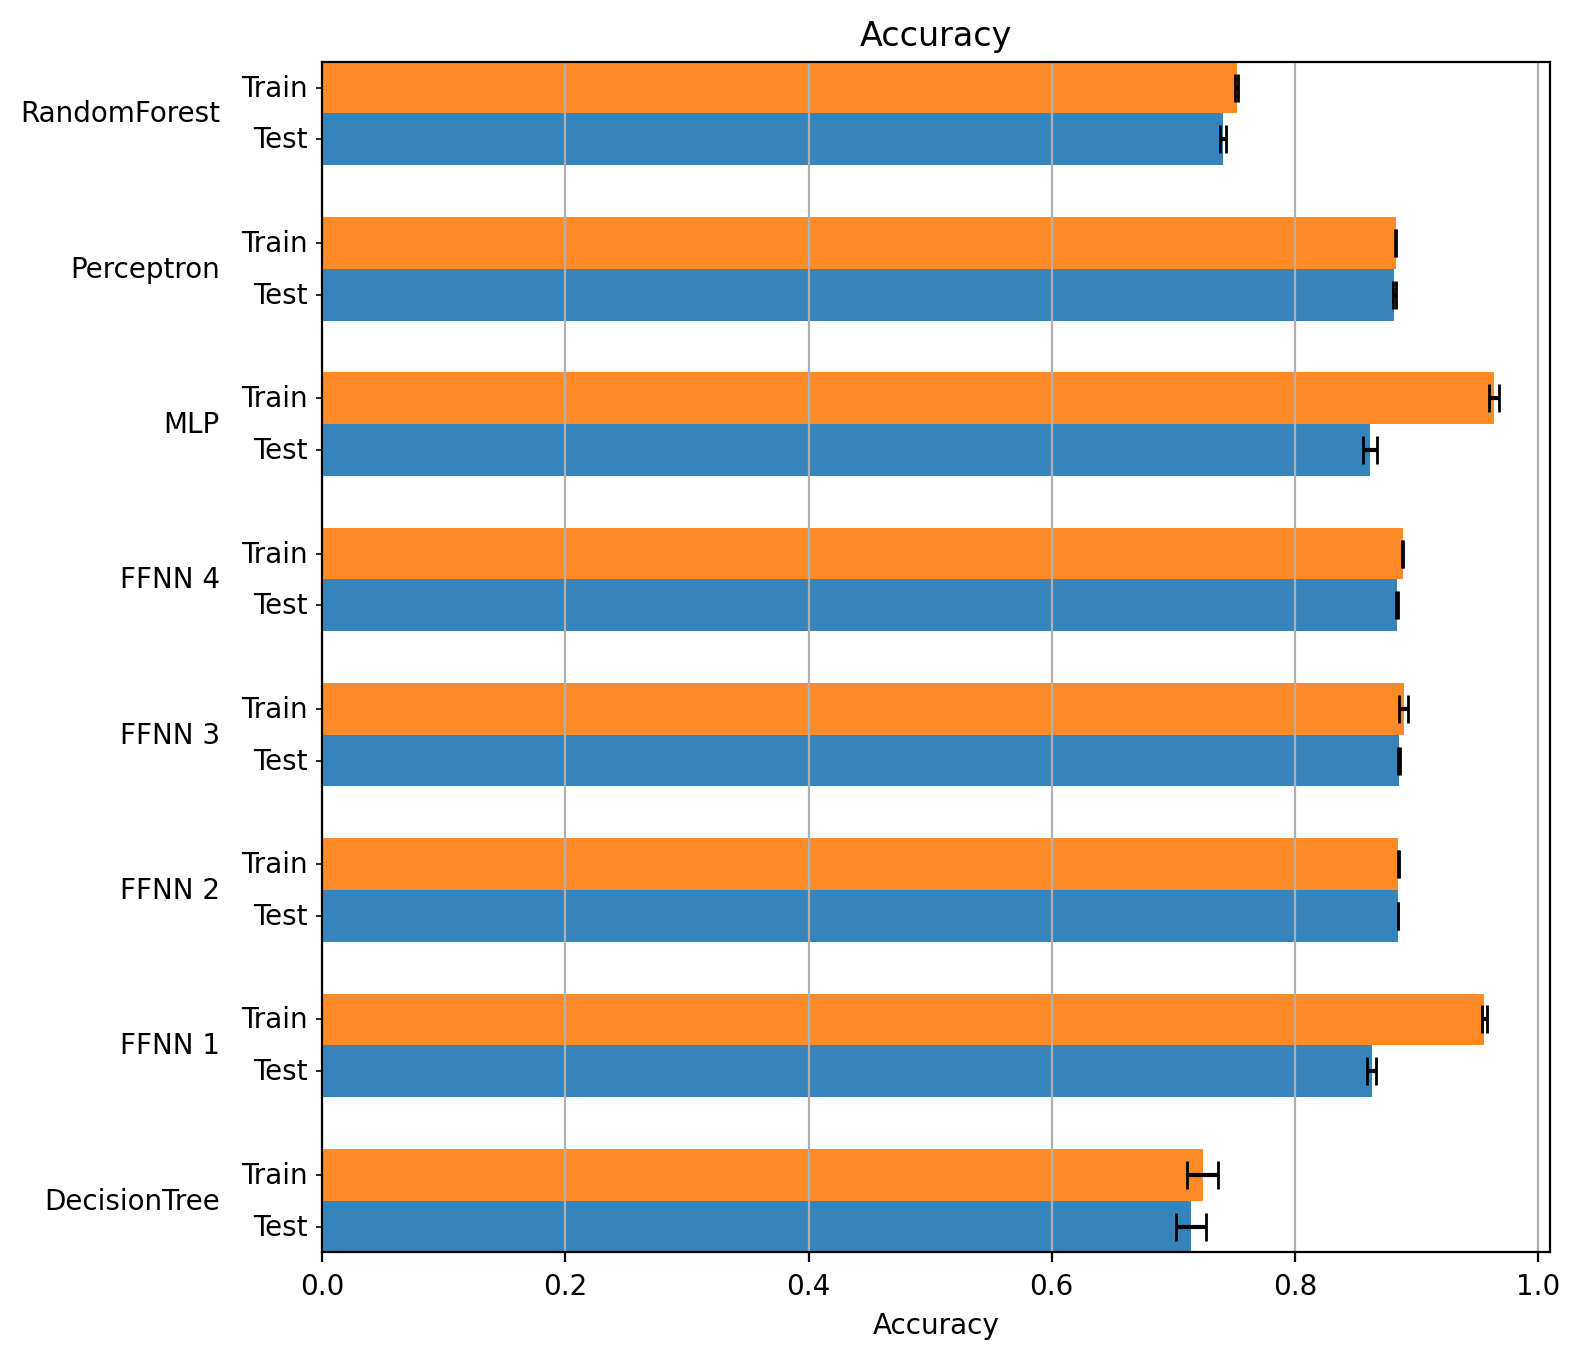
\includegraphics[width=0.77\linewidth]{../images/epigemomic_results/promoters/accuracy.png}
\caption{Accuracy metric for promoters epigenomic experiments}
\end{figure}

\textbf{AUROC}

\begin{longtable}[]{@{}lll@{}}
\toprule
\textbf{Models} & \textbf{Training} & \textbf{Test}\tabularnewline
\midrule
\endhead
DecisionTree & mean = 0.8081 & mean = 0.7862\tabularnewline
& STD = 0.0019 & STD = 0.0033\tabularnewline
RandomForest & mean = 0.8384 & mean = 0.8117\tabularnewline
& STD = 0.0008 & STD = 0.0027\tabularnewline
Perceptron & mean = 0.8674 & mean = 0.8638\tabularnewline
& STD = 0.0008 & STD = 0.0026\tabularnewline
MLP & mean = 0.9813 & mean = 0.8433\tabularnewline
& STD = 0.0014 & STD = 0.0054\tabularnewline
FFNN\_1 & mean = 0.9774 & mean = 0.8392\tabularnewline
& STD = 0.0016 & STD = 0.0057\tabularnewline
FFNN\_2 & mean = 0.9184 & mean = 0.8766\tabularnewline
& STD = 0.0039 & STD = 0.0028\tabularnewline
FFNN\_3 & mean = 0.9015 & mean = 0.8733\tabularnewline
& STD = 0.0103 & STD = 0.0042\tabularnewline
FFNN\_4 & mean = 0.8893 & mean = 0.8727\tabularnewline
& STD = 0.001 & STD = 0.0025\tabularnewline
\bottomrule
\end{longtable}

\begin{figure}[h!]
\centering
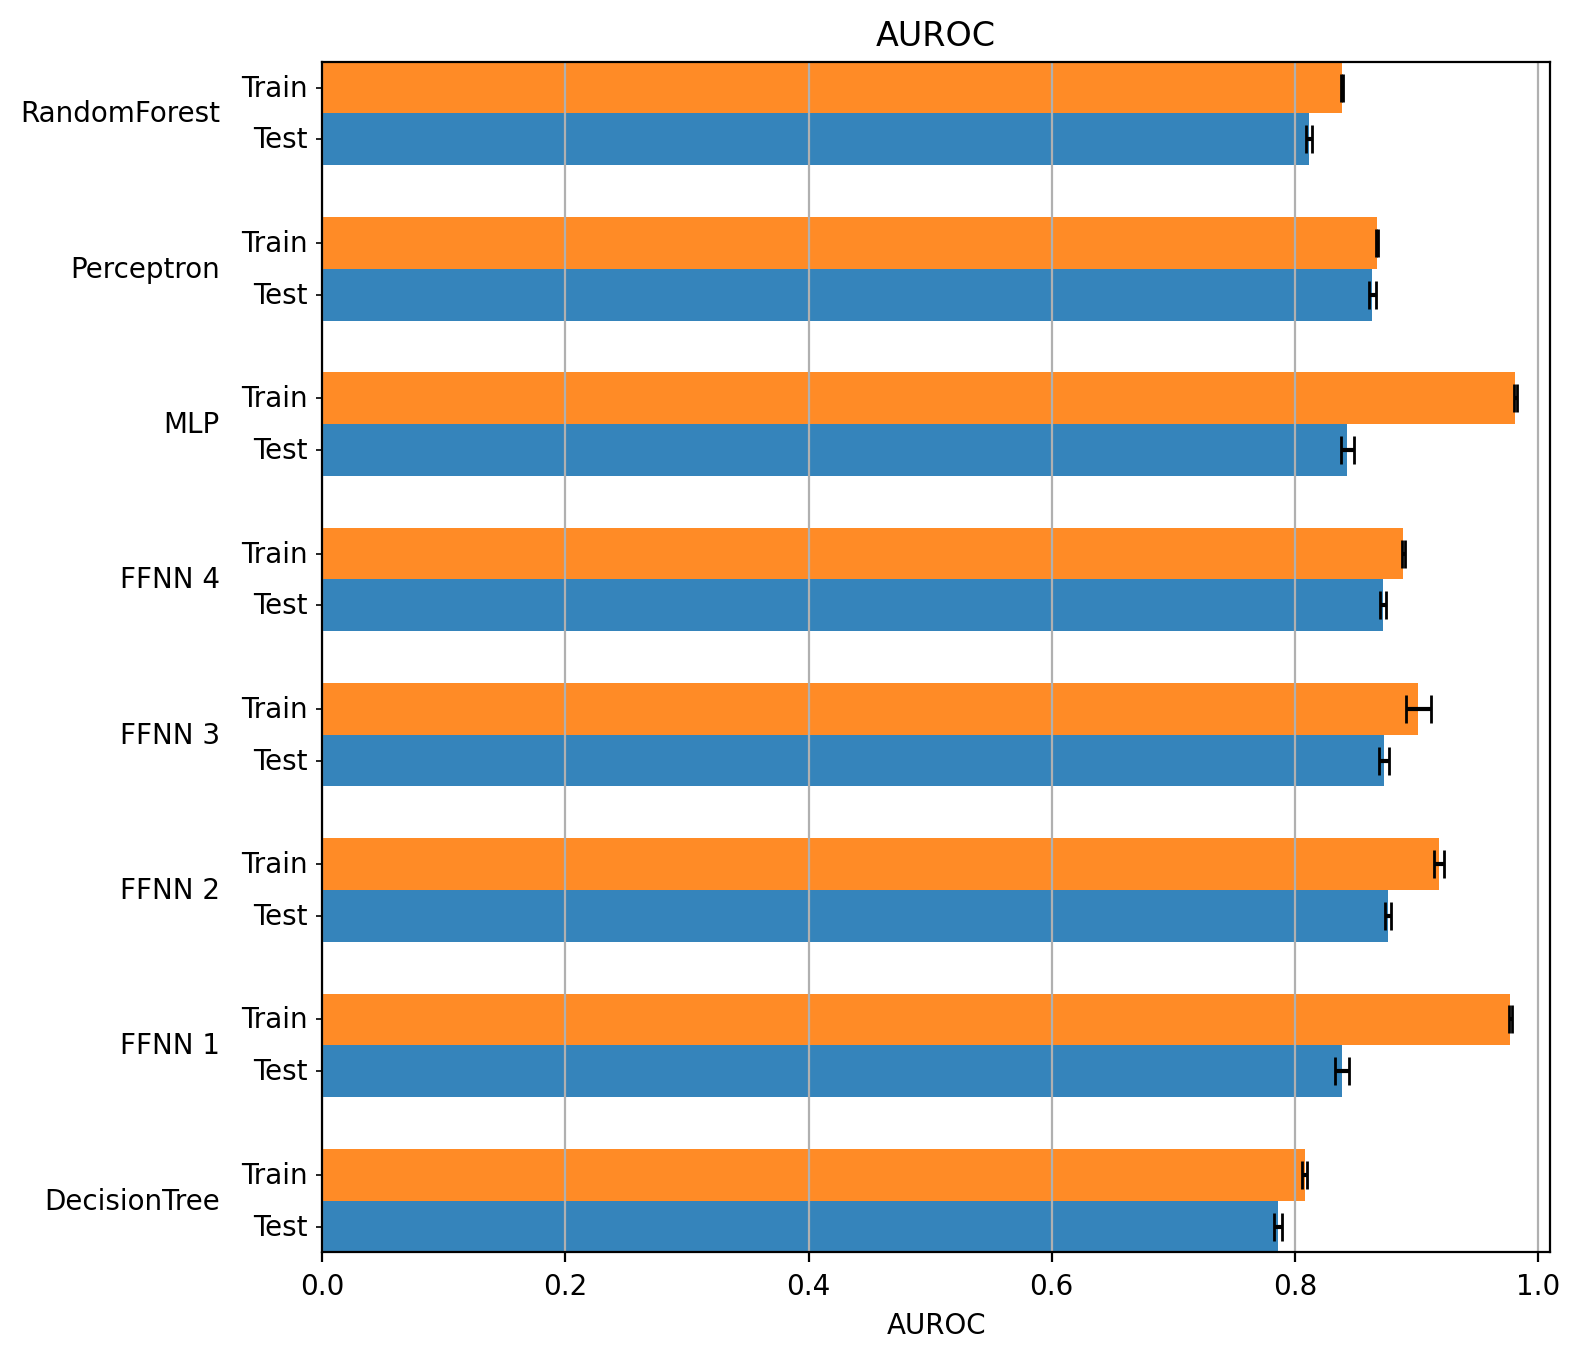
\includegraphics[width=0.77\linewidth]{../images/epigemomic_results/promoters/auroc.png}
\caption{AUROC metric for promoters epigenomic experiments}
\end{figure}

\textbf{AUPRC}

\begin{longtable}[]{@{}lll@{}}
\toprule
\textbf{Models} & \textbf{Training} & \textbf{Test}\tabularnewline
\midrule
\endhead
DecisionTree & mean = 0.2703 & mean = 0.2531\tabularnewline
& STD = 0.0046 & STD = 0.0037\tabularnewline
RandomForest & mean = 0.3018 & mean = 0.2784\tabularnewline
& STD = 0.0011 & STD = 0.0023\tabularnewline
Perceptron & mean = 0.3953 & mean = 0.3867\tabularnewline
& STD = 0.0022 & STD = 0.0077\tabularnewline
MLP & mean = 0.8998 & mean = 0.3524\tabularnewline
& STD = 0.0089 & STD = 0.011\tabularnewline
FFNN\_1 & mean = 0.878 & mean = 0.3459\tabularnewline
& STD = 0.0082 & STD = 0.0082\tabularnewline
FFNN\_2 & mean = 0.496 & mean = 0.4245\tabularnewline
& STD = 0.0145 & STD = 0.009\tabularnewline
FFNN\_3 & mean = 0.5009 & mean = 0.4146\tabularnewline
& STD = 0.0384 & STD = 0.0092\tabularnewline
FFNN\_4 & mean = 0.4632 & mean = 0.4047\tabularnewline
& STD = 0.0053 & STD = 0.0076\tabularnewline
\bottomrule
\end{longtable}

\begin{figure}[h!]
\centering
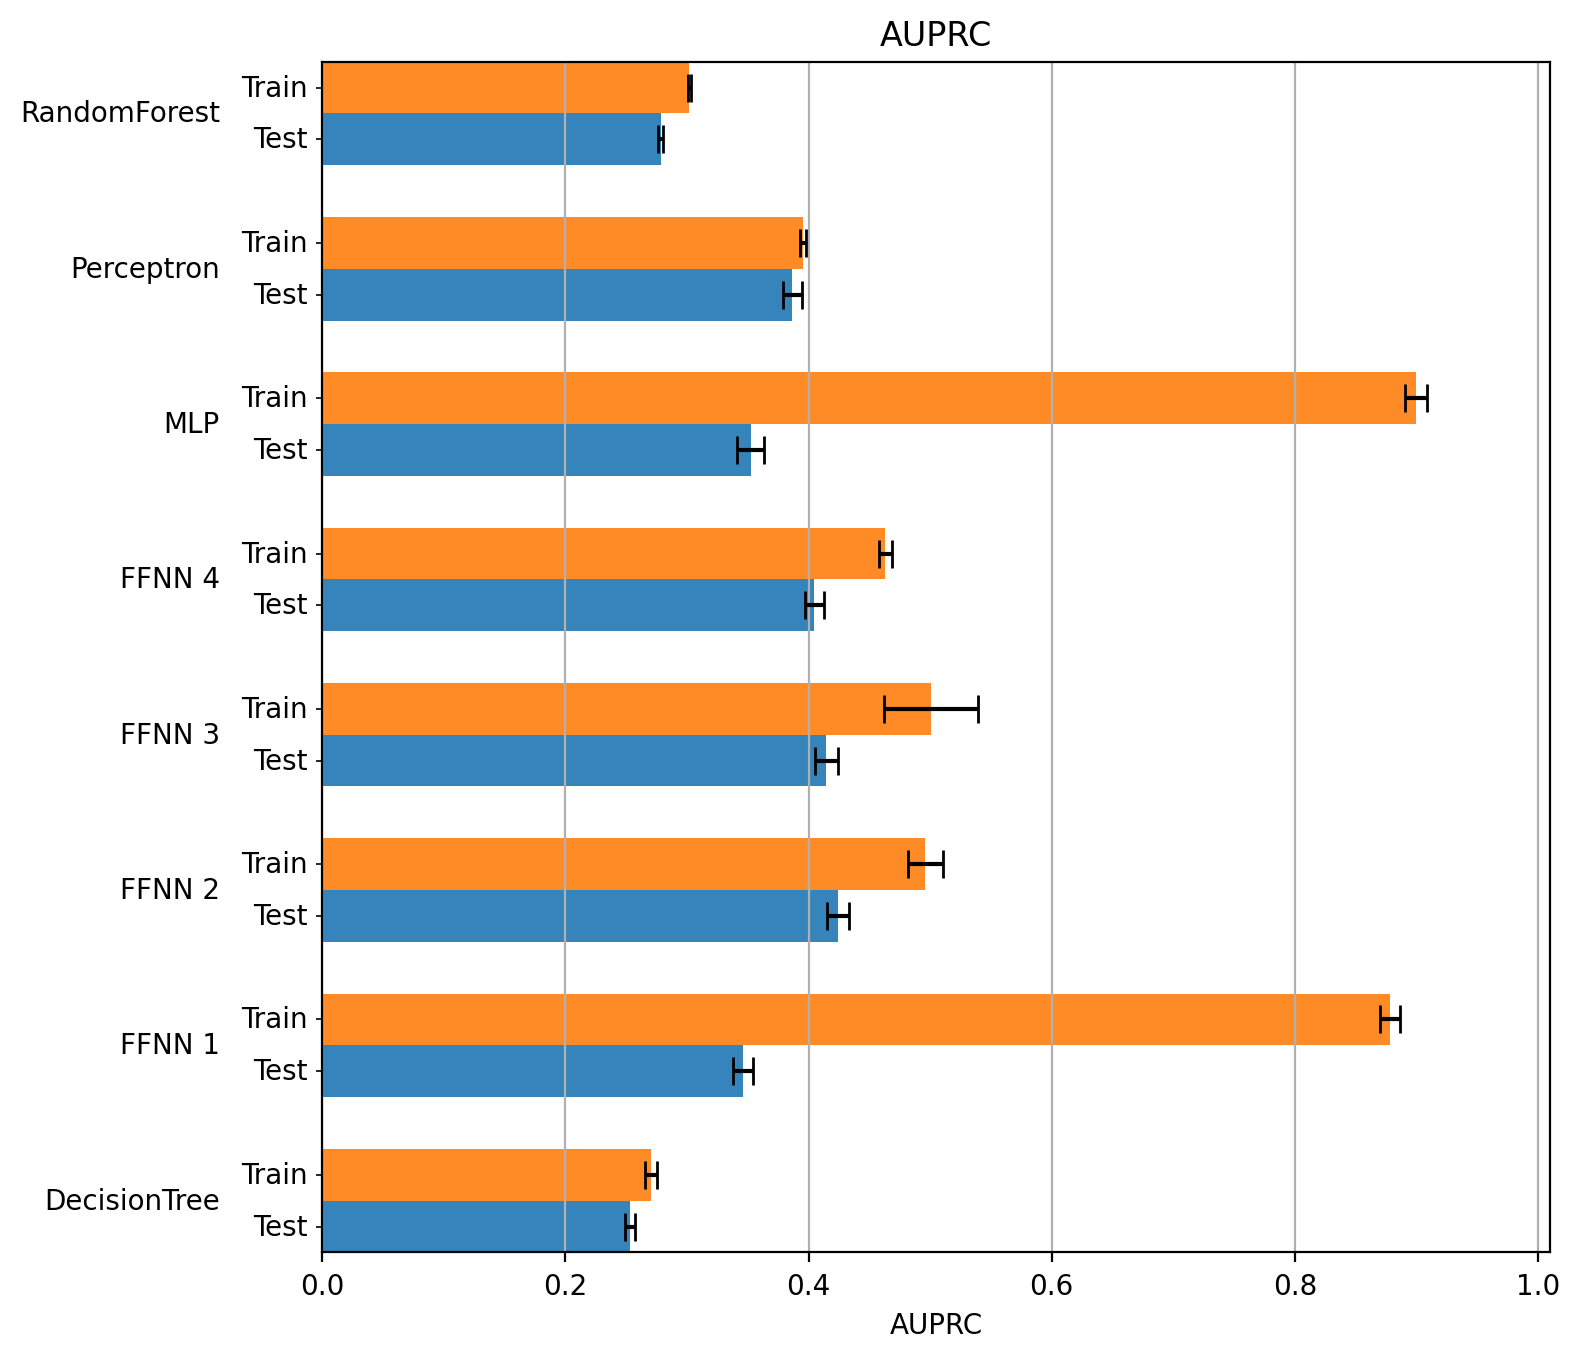
\includegraphics[width=0.77\linewidth]{../images/epigemomic_results/promoters/auprc.png}
\caption{AUPRC metric for promoters epigenomic experiments}
\end{figure}

\subsubsection{Enhancers}

In this section are reported the experiment results for active vs
inactive enhancers task using epigenomic data. For each metric there are
a table and a plot to confront the learning machine performance.

\textbf{Accuracy}

\begin{longtable}[]{@{}lll@{}}
	\toprule
	\textbf{Models} & \textbf{Training} & \textbf{Test}\tabularnewline
	\midrule
	\endhead
	DecisionTree & mean = 0.7417 & mean = 0.7316\tabularnewline
	& STD = 0.0303 & STD = 0.0297\tabularnewline
	RandomForest & mean = 0.8248 & mean = 0.8144\tabularnewline
	& STD = 0.0023 & STD = 0.0037\tabularnewline
	Perceptron & mean = 0.8978 & mean = 0.897\tabularnewline
	& STD = 0.0003 & STD = 0.0009\tabularnewline
	MLP & mean = 0.9793 & mean = 0.8545\tabularnewline
	& STD = 0.0142 & STD = 0.0108\tabularnewline
	FFNN\_1 & mean = 0.9784 & mean = 0.8501\tabularnewline
	& STD = 0.0014 & STD = 0.0046\tabularnewline
	FFNN\_2 & mean = 0.8964 & mean = 0.8958\tabularnewline
	& STD = 0.0012 & STD = 0.0009\tabularnewline
	FFNN\_3 & mean = 0.8991 & mean = 0.8971\tabularnewline
	& STD = 0.0015 & STD = 0.0009\tabularnewline
	FFNN\_4 & mean = 0.9021 & mean = 0.8978\tabularnewline
	& STD = 0.0004 & STD = 0.001\tabularnewline
	\bottomrule
\end{longtable}

\begin{figure}[h!]
	\centering
	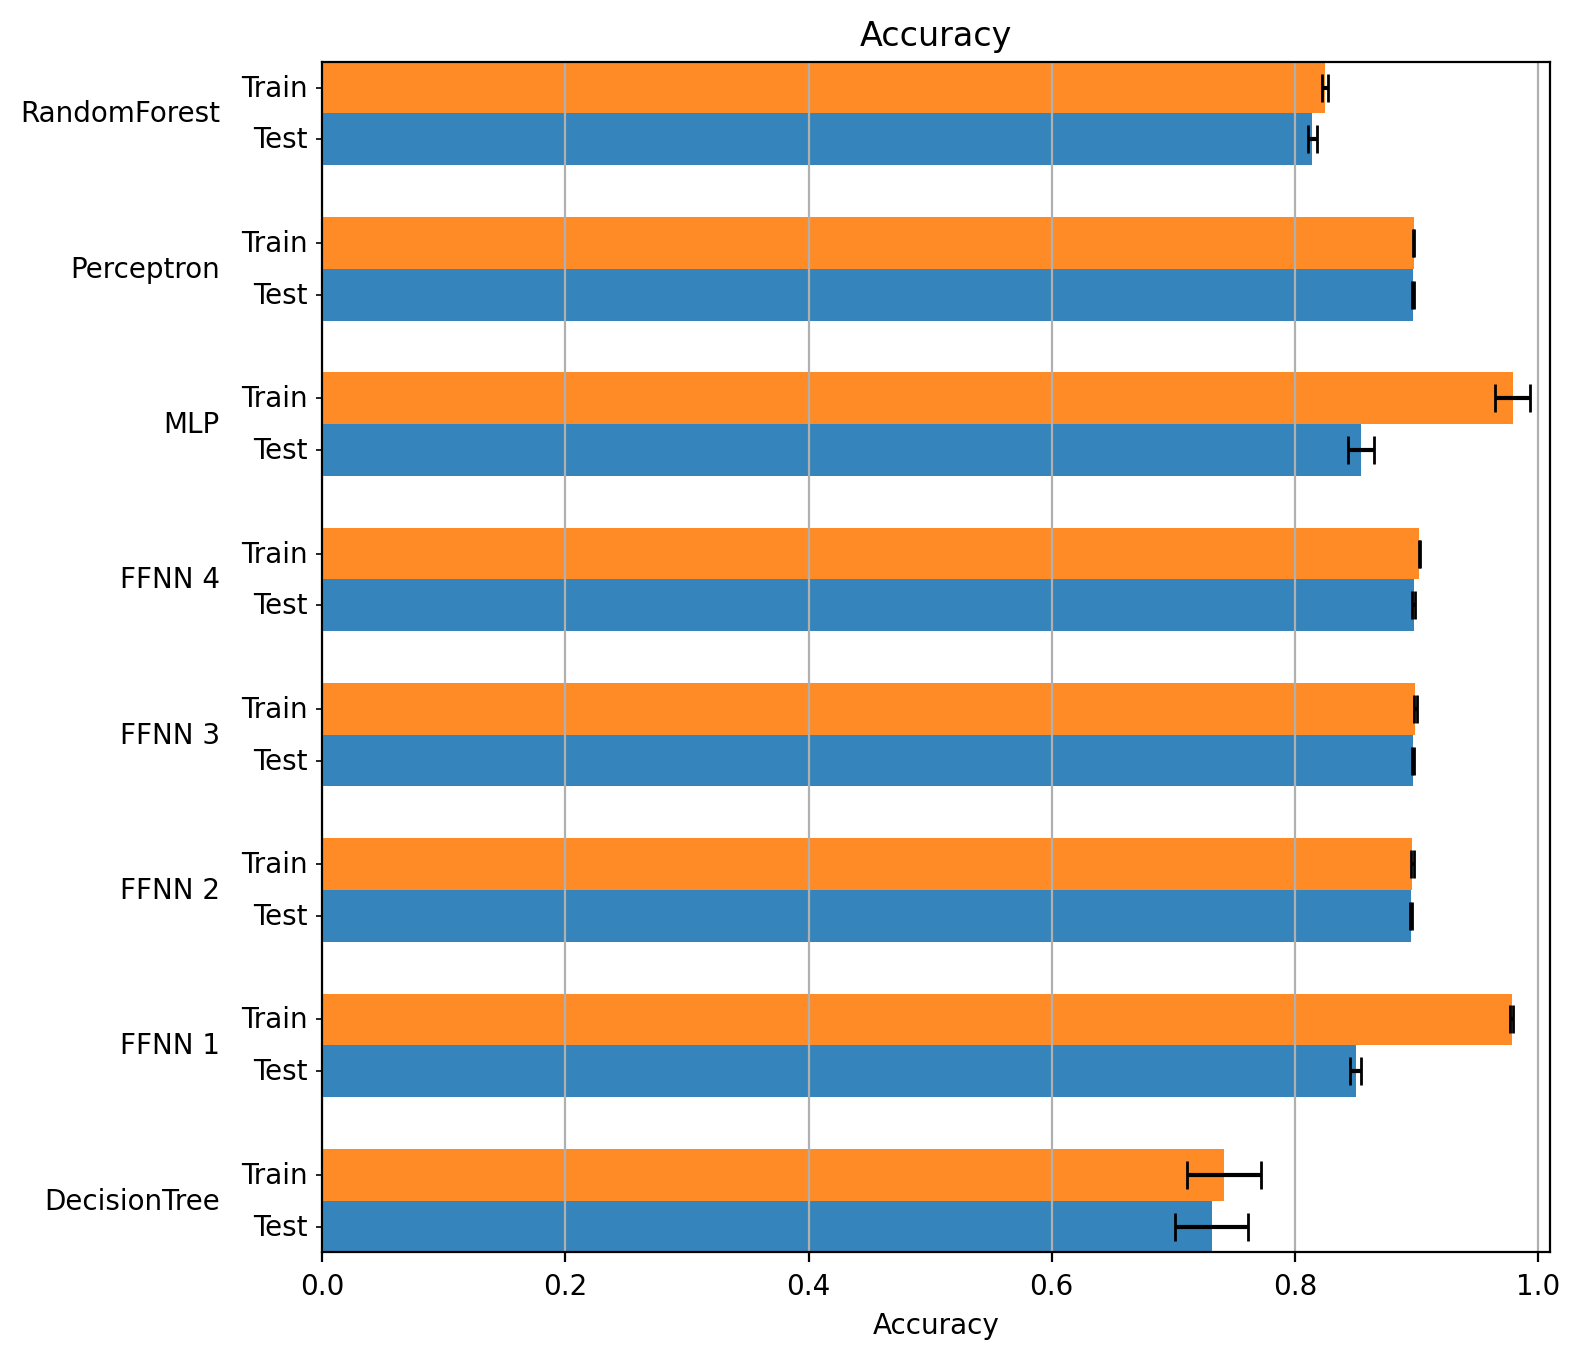
\includegraphics[width=0.6\linewidth]{../images/epigemomic_results/enhancers/accuracy.png}
	\caption{Accuracy metric for enhancers epigenomic experiments}
\end{figure}

\textbf{AUROC}

\begin{longtable}[]{@{}lll@{}}
	\toprule
	\textbf{Models} & \textbf{Training} & \textbf{Test}\tabularnewline
	\midrule
	\endhead
	DecisionTree & mean = 0.6453 & mean = 0.6168\tabularnewline
	& STD = 0.0029 & STD = 0.0067\tabularnewline
	RandomForest & mean = 0.6521 & mean = 0.626\tabularnewline
	& STD = 0.0017 & STD = 0.006\tabularnewline
	Perceptron & mean = 0.6903 & mean = 0.6796\tabularnewline
	& STD = 0.002 & STD = 0.0071\tabularnewline
	MLP & mean = 0.9608 & mean = 0.6097\tabularnewline
	& STD = 0.0263 & STD = 0.0109\tabularnewline
	FFNN\_1 & mean = 0.9652 & mean = 0.6136\tabularnewline
	& STD = 0.0017 & STD = 0.0083\tabularnewline
	FFNN\_2 & mean = 0.8646 & mean = 0.6703\tabularnewline
	& STD = 0.0124 & STD = 0.008\tabularnewline
	FFNN\_3 & mean = 0.7462 & mean = 0.6833\tabularnewline
	& STD = 0.0206 & STD = 0.0062\tabularnewline
	FFNN\_4 & mean = 0.7284 & mean = 0.6816\tabularnewline
	& STD = 0.0027 & STD = 0.0068\tabularnewline
	\bottomrule
\end{longtable}

\begin{figure}[h!]
	\centering
	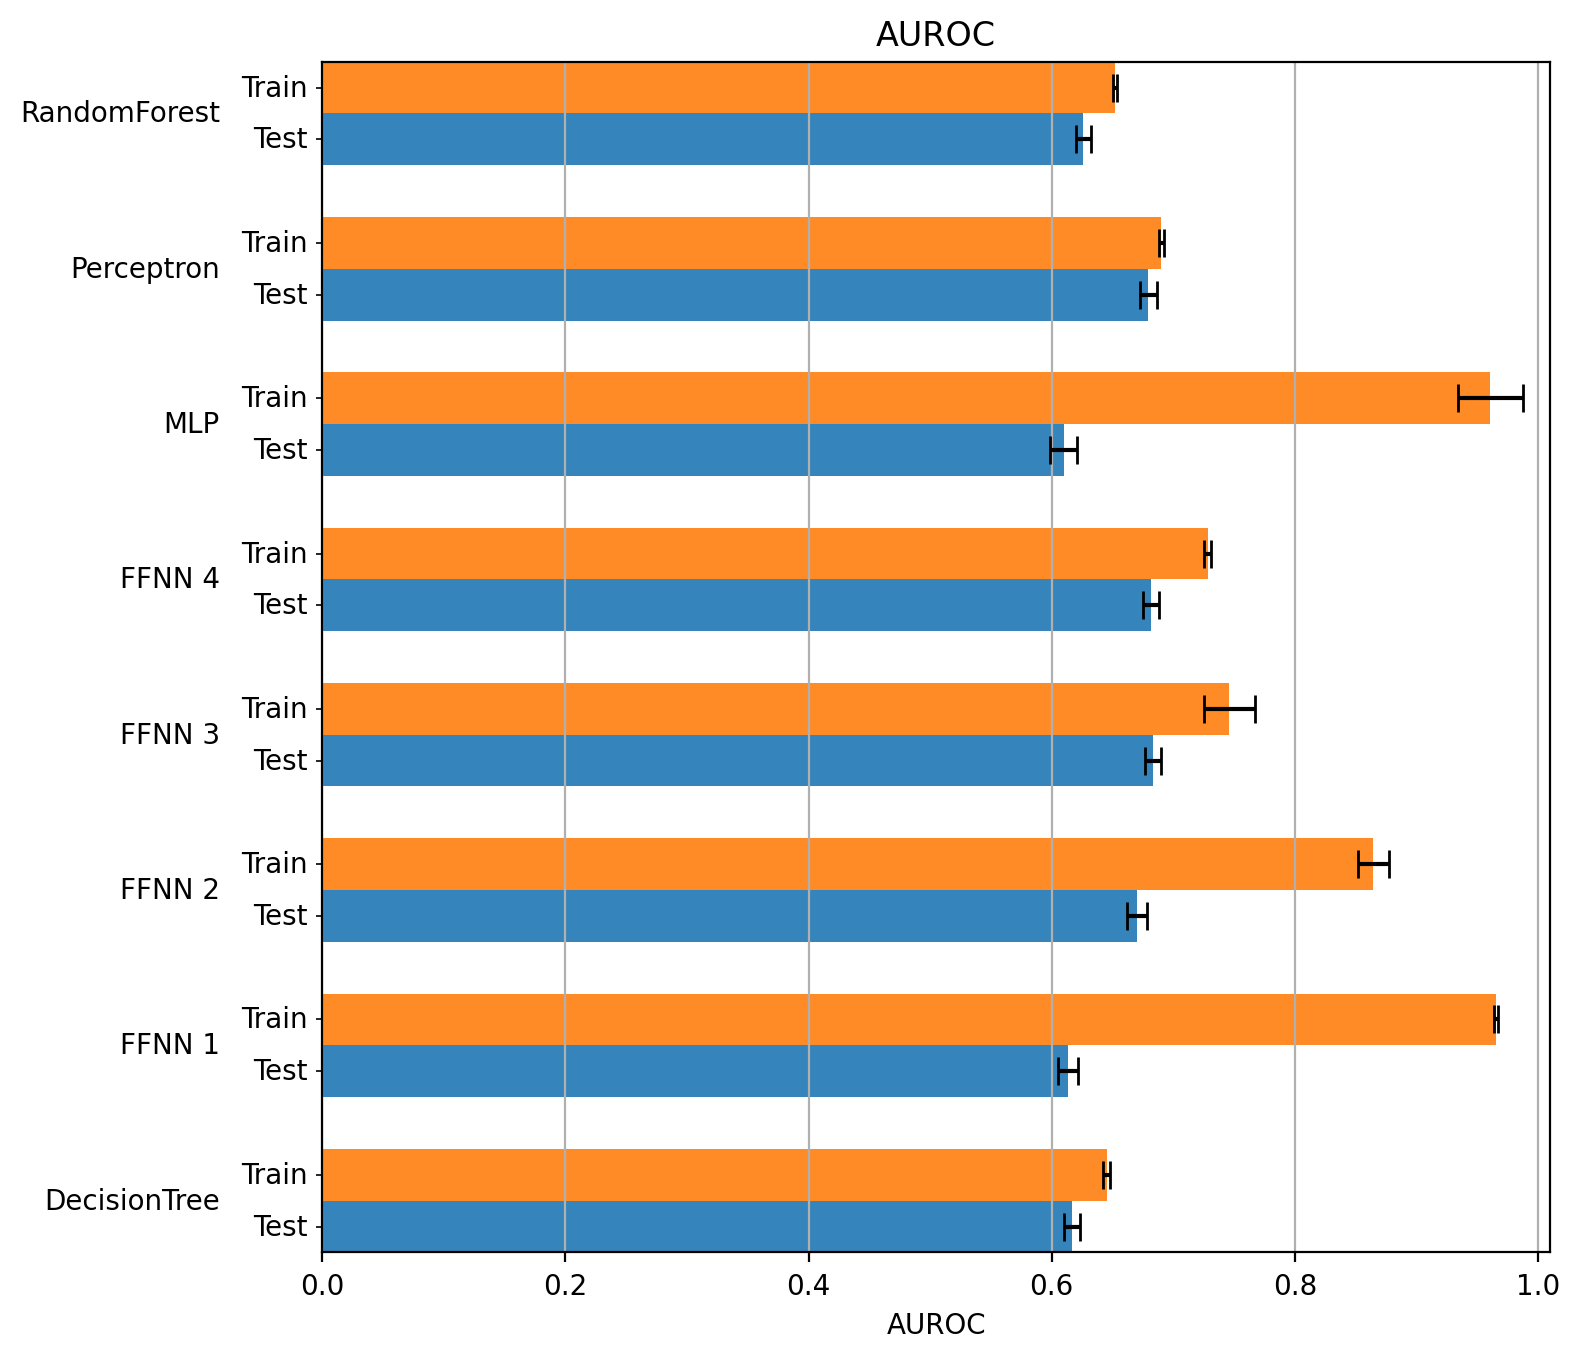
\includegraphics[width=0.77\linewidth]{../images/epigemomic_results/enhancers/auroc.png}
	\caption{AUROC metric for enhancers epigenomic experiments}
\end{figure}

\textbf{AUPRC}

\begin{longtable}[]{@{}lll@{}}
	\toprule
	\textbf{Models} & \textbf{Training} & \textbf{Test}\tabularnewline
	\midrule
	\endhead
	DecisionTree & mean = 0.1617 & mean = 0.1464\tabularnewline
	& STD = 0.0045 & STD = 0.004\tabularnewline
	RandomForest & mean = 0.184 & mean = 0.1636\tabularnewline
	& STD = 0.0012 & STD = 0.004\tabularnewline
	Perceptron & mean = 0.2964 & mean = 0.2852\tabularnewline
	& STD = 0.0029 & STD = 0.0103\tabularnewline
	MLP & mean = 0.9059 & mean = 0.1867\tabularnewline
	& STD = 0.0803 & STD = 0.0137\tabularnewline
	FFNN\_1 & mean = 0.9187 & mean = 0.1726\tabularnewline
	& STD = 0.0039 & STD = 0.0088\tabularnewline
	FFNN\_2 & mean = 0.452 & mean = 0.2824\tabularnewline
	& STD = 0.0255 & STD = 0.0118\tabularnewline
	FFNN\_3 & mean = 0.3494 & mean = 0.2901\tabularnewline
	& STD = 0.0202 & STD = 0.0116\tabularnewline
	FFNN\_4 & mean = 0.3558 & mean = 0.2858\tabularnewline
	& STD = 0.0042 & STD = 0.011\tabularnewline
	\bottomrule
\end{longtable}

\begin{figure}[h!]
	\centering
	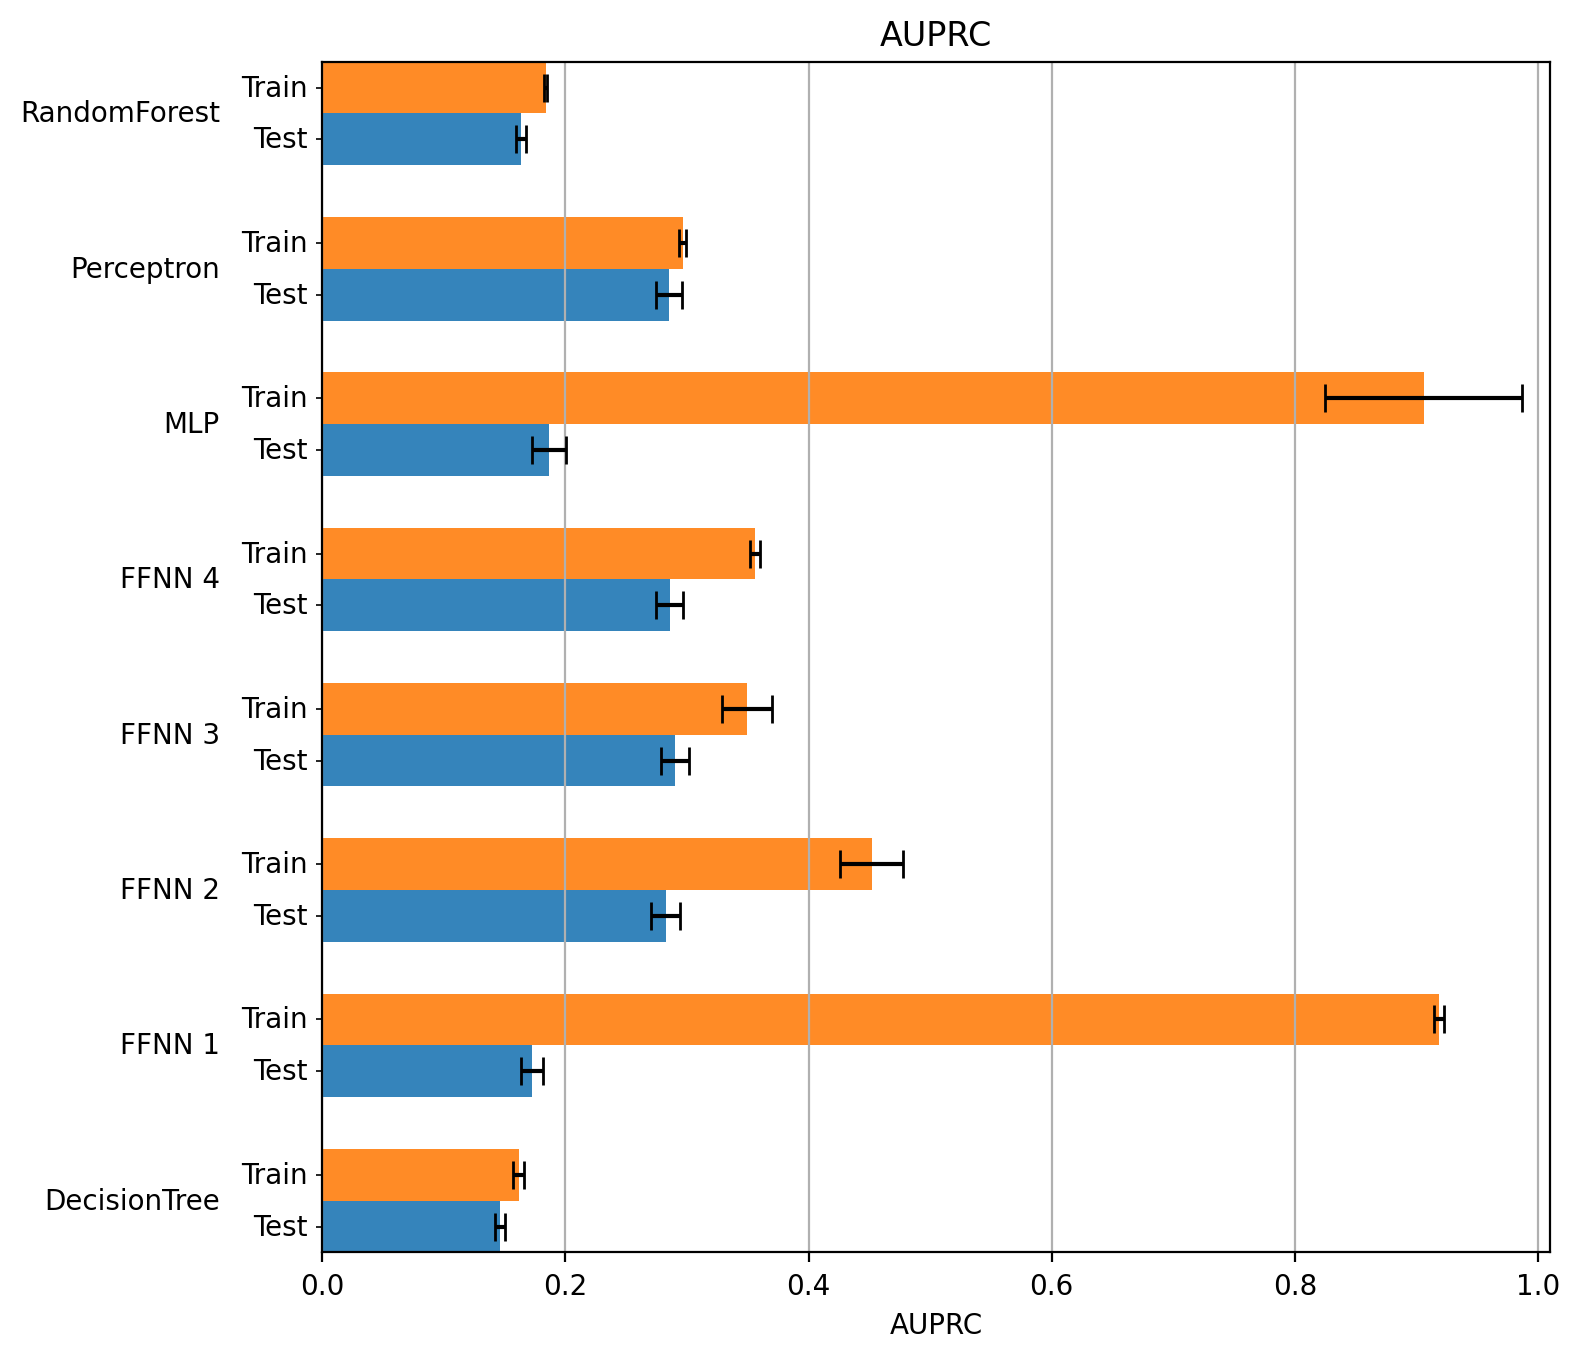
\includegraphics[width=0.77\linewidth]{../images/epigemomic_results/enhancers/auprc.png}
	\caption{AUPRC metric for enhancers epigenomic experiments}
\end{figure}
\subsubsection{Observations}
\paragraph{Promoters' obervations}
The following observations refer to the experiments executed on the promoters' epigenomic data.
\newline
\par
\emph{1) DecisionTree and RandomForest perform worst than other models.}
The results show that DecisionTree and Random Forest perform worst than
the other models according to all metrics, both for promoters and
enhancers.

\emph{2) There is a big problem of overfitting with complex deep
networks.} The data decomposition graphs show that the promoters'
epigenomic data are not clearly separable and the complex models tend to
learn data without generalizing. This happens in particular with the MLP
and FFNN\_1 and it is visible in the AUPRC metric.

\emph{3) The perceptron performance is comparable with more complex
models.} This model indeed does not overfit because of its very simple
structure and it can better generalize. In particular, according to the
Wilcoxon test, the perceptron performs better than DecisionTree,
RandomForest, MLP, and FFNN\_1 in all metrics.

\emph{4) The FFNN\_3 does not improve the performance despite it tries to
resolve the class imbalance problem.} The measures adopted have only
prevented overfitting but the test result is not the best. Besides,
FFNN\_3 has the largest STD in the training results according to all
metrics.

\emph{5) FFNN\_2 is the best model.} According to the Wilcoxon test,
this model performs better than the others in all metrics, except for
the FFNN\_3 according to the accuracy. This model has a complex
architecture, composed of 5 hidden layers and a big dropout for each of
them. This strategy allows the network to learn the data without
overfitting.

\emph{6) All models fail to recognize the positive samples.} The
accuracy and AUROC are high and they hide the real model performances.
This is because the dataset is unbalanced (the positive samples
represent the minority class) and these metrics do not capture the fact
that the model correctly classifies only a few part of the positive
samples. Thanks to the AUPRC, it is evident that the models produce a
lot of false-negative because this metric is always less than 0.5.
\newline
\paragraph{Enhancers' obervations}
The following observations refer to the experiments executed on the enhancers' epigenomic data.
\newline
\par
\emph{1) DecisionTree and RandomForest perform worst than other models.}
The results show that DecisionTree and Random Forest perform worst than
the other models according to all metrics, both for promoters and
enhancers.

\emph{2) The overfitting problem is more pronounced than promoters.} The
data decomposition graphs show that the enhancers' epigenomic data are
not clearly separable and the complex models tend to learn data without
generalizing. This happens in particular with the MLP and FFNN\_1 and it
is visible in the AUPRC metric.

\emph{3) The perceptron performance is comparable with more complex
models.} This model indeed does not overfit because of its very simple
structure and it can better generalize. In particular, according to the
Wilcoxon test, the perceptron performs better than DecisionTree,
RandomForest, MLP, and FFNN\_1. Also, the FFNN\_2 is worst than
perceptron according to accuracy and AUROC, while for AUPRC these two
models are statistically identical.

\emph{4) The reduction of overfitting does not improve performance.}
Unlike promoters' experiments, the networks are not able to better
generalize despite the reduction of the training metrics values. The
enhancers' epigenomic data are less separable than promoters' ones, as
shown by PCA and TSNE data decomposition graphs. Moreover, the enhancers
have fewer samples than the promoters and the data imbalance is more
pronounced.

\emph{5) There isn't the best model.} The deep networks tested for
enhancers win and loose according to various metrics. For accuracy, the
best model is the FFNN\_4. Despite according to the AUROC, the
models that perform better are FFNN\_3 and FFNN\_4: they are
statistically identical. Finally, for AUPRC, the FFNN\_3 is the best
model.
\newpage
\subsection{Sequence experiments}

\subsubsection{Promoters}

\textbf{Accuracy}

\begin{longtable}[]{@{}lll@{}}
\toprule
\textbf{Models} & \textbf{Training} & \textbf{Test}\tabularnewline
\midrule
\endhead
Perceptron & mean = 0.8848 & mean = 0.8847\tabularnewline
& STD = 0.0 & STD = 0.0\tabularnewline
MLP & mean = 0.983 & mean = 0.8\tabularnewline
& STD = 0.0132 & STD = 0.0071\tabularnewline
FFNN\_1 & mean = 0.9984 & mean = 0.8188\tabularnewline
& STD = 0.0001 & STD = 0.0006\tabularnewline
CNN\_1 & mean = 0.9719 & mean = 0.8381\tabularnewline
& STD = 0.0008 & STD = 0.0017\tabularnewline
CNN\_2 & mean = 0.9918 & mean = 0.807\tabularnewline
& STD = 0.0021 & STD = 0.0187\tabularnewline
CNN\_3 & mean = 0.956 & mean = 0.8641\tabularnewline
& STD = 0.0504 & STD = 0.0146\tabularnewline
\bottomrule
\end{longtable}

\begin{figure}[h!]
\centering
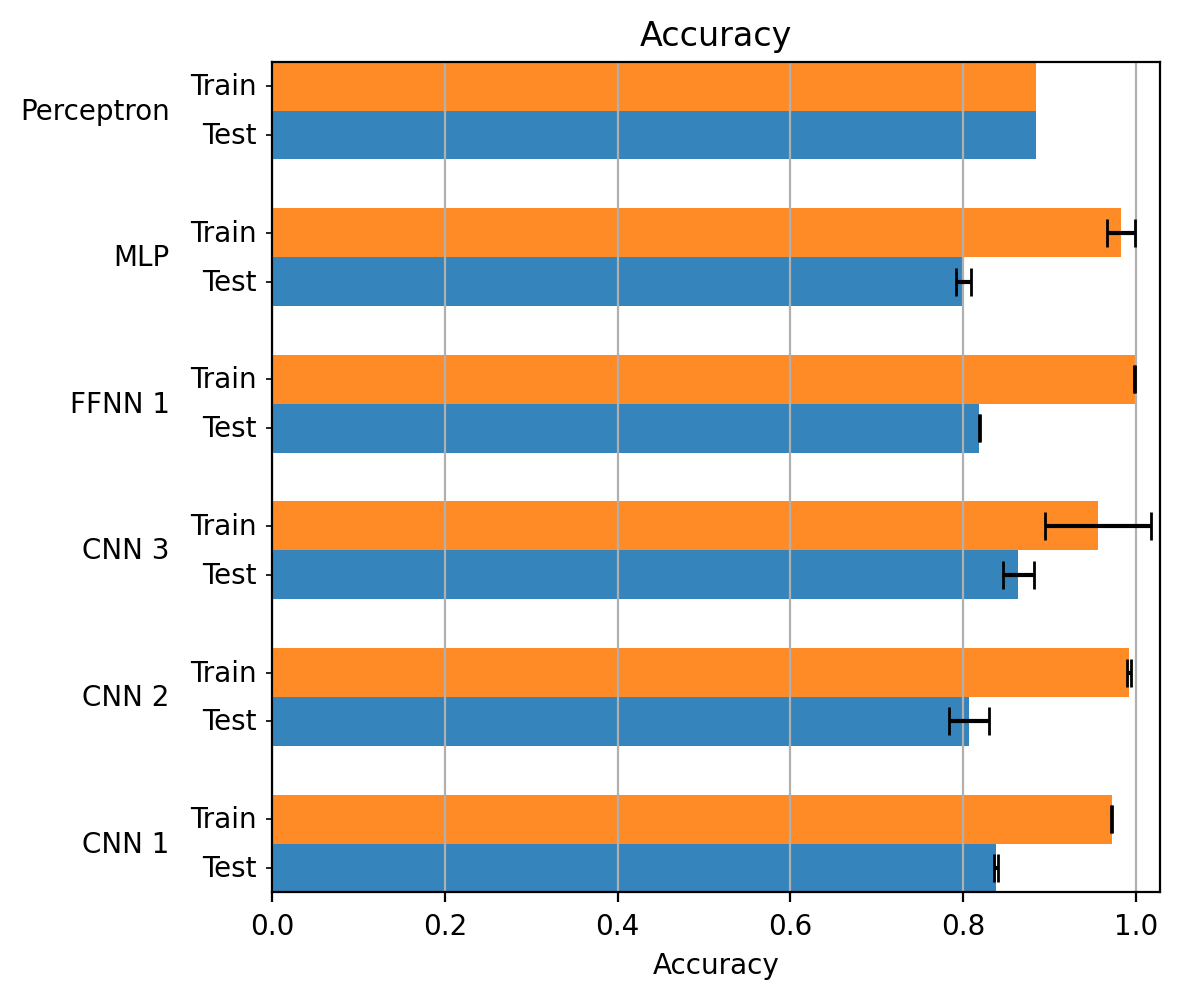
\includegraphics[width=0.8\linewidth]{../images/sequence_results/promoters/accuracy.png}
\caption{Accuracy metric for promoters sequence experiments}
\end{figure}

\textbf{AUROC}

\begin{longtable}[]{@{}lll@{}}
\toprule
\textbf{Models} & \textbf{Training} & \textbf{Test}\tabularnewline
\midrule
\endhead
Perceptron & mean = 0.5622 & mean = 0.5031\tabularnewline
& STD = 0.0027 & STD = 0.0024\tabularnewline
MLP & mean = 0.9933 & mean = 0.5049\tabularnewline
& STD = 0.0079 & STD = 0.005\tabularnewline
FFNN\_1 & mean = 0.9998 & mean = 0.5039\tabularnewline
& STD = 0.0 & STD = 0.003\tabularnewline
CNN\_1 & mean = 0.9893 & mean = 0.4914\tabularnewline
& STD = 0.0008 & STD = 0.0076\tabularnewline
CNN\_2 & mean = 0.9973 & mean = 0.5003\tabularnewline
& STD = 0.0006 & STD = 0.0052\tabularnewline
CNN\_3 & mean = 0.8313 & mean = 0.5006\tabularnewline
& STD = 0.2349 & STD = 0.0035\tabularnewline
\bottomrule
\end{longtable}

\begin{figure}[h!]
\centering
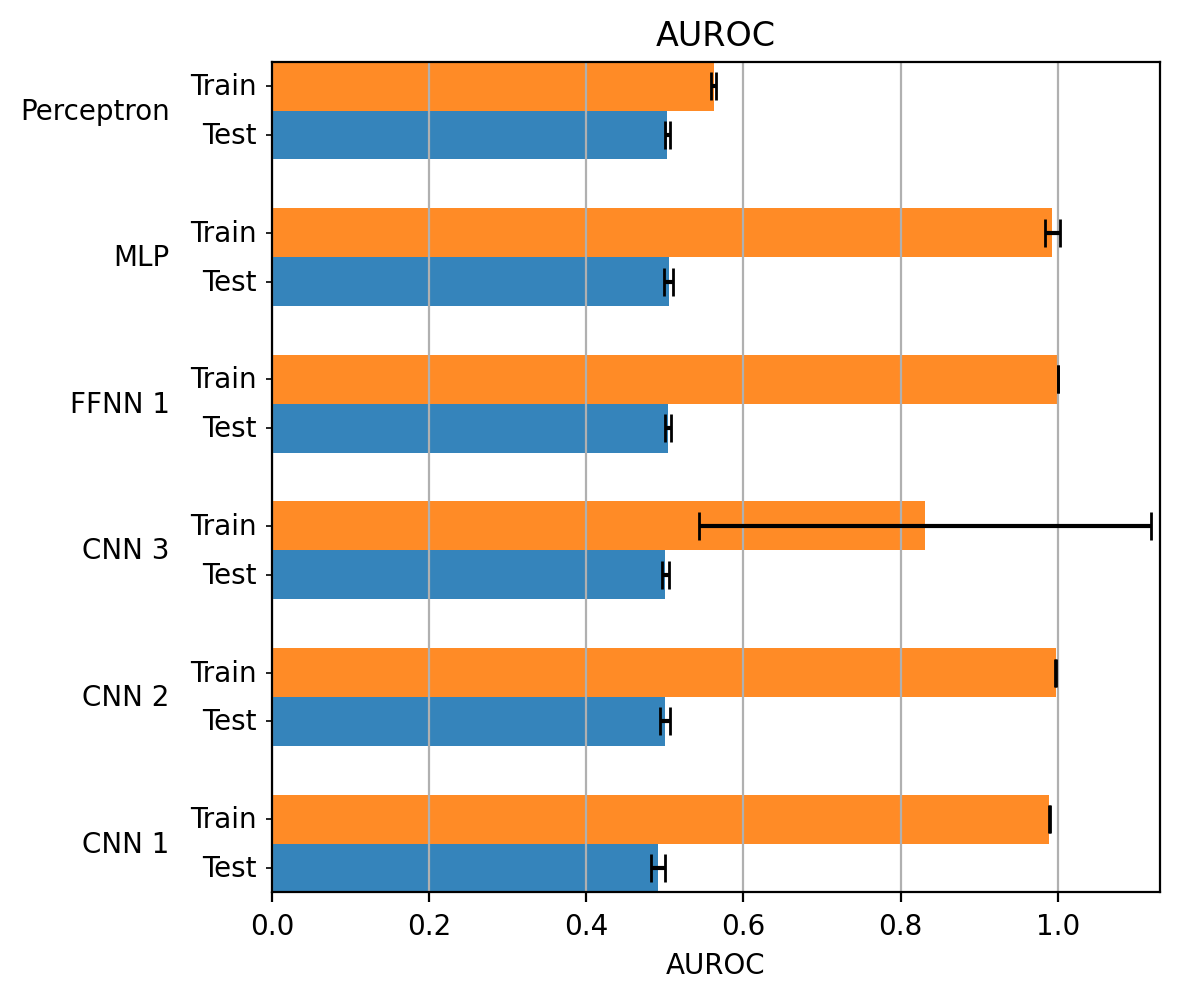
\includegraphics[width=0.8\linewidth]{../images/sequence_results/promoters/auroc.png}
\caption{AUROC metric for promoters sequence experiments}
\end{figure}
\newpage
\textbf{AUPRC}

\begin{longtable}[]{@{}lll@{}}
\toprule
\textbf{Models} & \textbf{Training} & \textbf{Test}\tabularnewline
\midrule
\endhead
Perceptron & mean = 0.14 & mean = 0.116\tabularnewline
& STD = 0.0026 & STD = 0.0013\tabularnewline
MLP & mean = 0.9697 & mean = 0.1176\tabularnewline
& STD = 0.0345 & STD = 0.0014\tabularnewline
FFNN\_1 & mean = 0.9991 & mean = 0.1175\tabularnewline
& STD = 0.0001 & STD = 0.001\tabularnewline
CNN\_1 & mean = 0.9472 & mean = 0.1126\tabularnewline
& STD = 0.0031 & STD = 0.0026\tabularnewline
CNN\_2 & mean = 0.9843 & mean = 0.1155\tabularnewline
& STD = 0.0025 & STD = 0.0017\tabularnewline
CNN\_3 & mean = 0.6925 & mean = 0.1153\tabularnewline
& STD = 0.4083 & STD = 0.0012\tabularnewline
\bottomrule
\end{longtable}

\begin{figure}[h!]
\centering
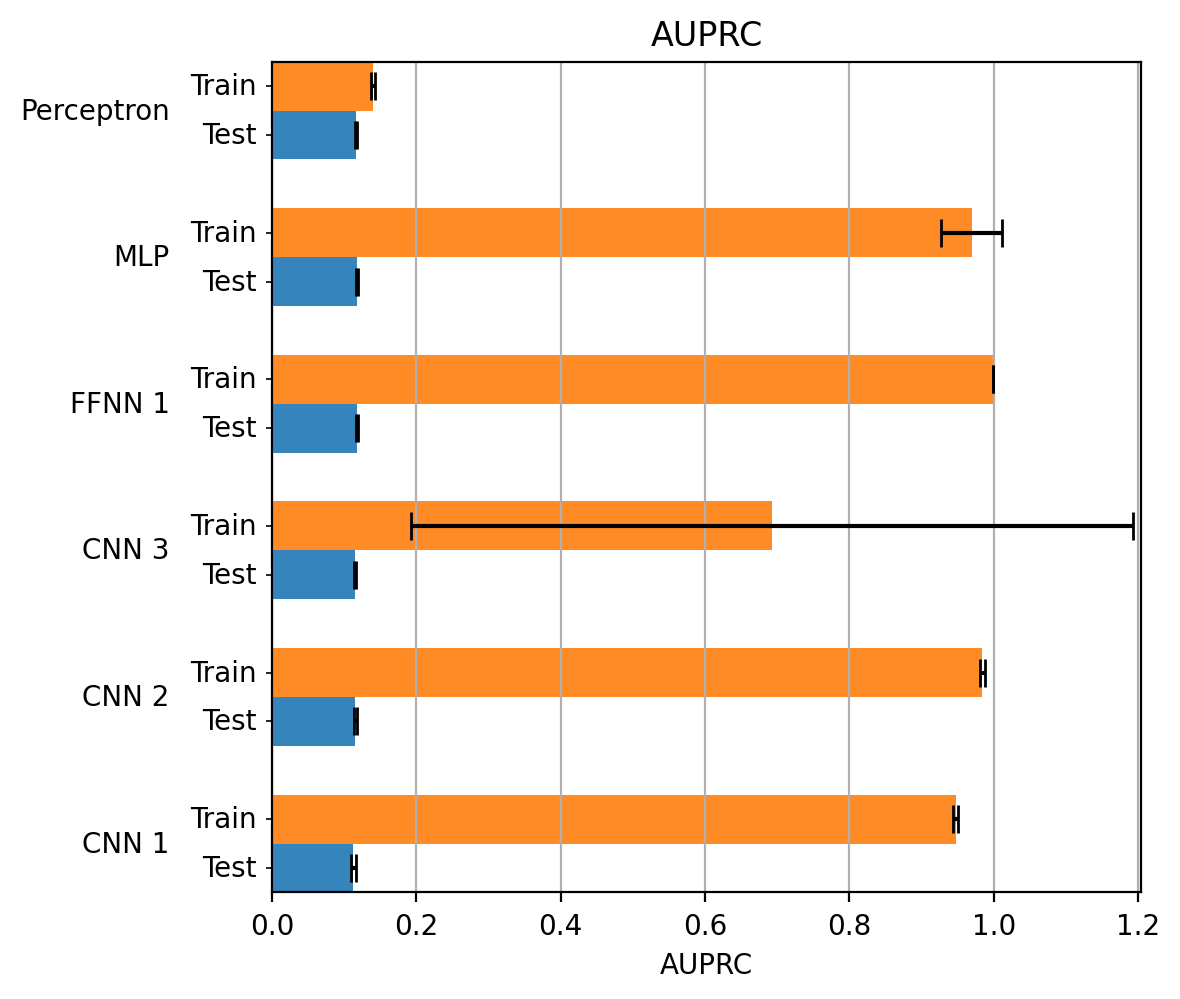
\includegraphics[width=0.8\linewidth]{../images/sequence_results/promoters/auprc.png}
\caption{AUPRC metric for promoters sequence experiments}
\end{figure}

\subsubsection{Enhancers}\label{header-n1661}

\textbf{Accuracy}

\begin{longtable}[]{@{}lll@{}}
\toprule
\textbf{Models} & \textbf{Training} & \textbf{Test}\tabularnewline
\midrule
\endhead
Perceptron & mean = 0.8937 & mean = 0.8938\tabularnewline
& STD = 0.0 & STD = 0.0\tabularnewline
MLP & mean = 1.0 & mean = 0.8245\tabularnewline
& STD = 0.0 & STD = 0.0022\tabularnewline
FFNN\_1 & mean = 0.9991 & mean = 0.8424\tabularnewline
& STD = 0.0006 & STD = 0.0033\tabularnewline
CNN\_1 & mean = 0.987 & mean = 0.8504\tabularnewline
& STD = 0.0013 & STD = 0.0175\tabularnewline
CNN\_2 & mean = 0.9916 & mean = 0.8146\tabularnewline
& STD = 0.0047 & STD = 0.0489\tabularnewline
CNN\_3 & mean = 0.9948 & mean = 0.8667\tabularnewline
& STD = 0.0001 & STD = 0.0028\tabularnewline
\bottomrule
\end{longtable}

\begin{figure}[h!]
\centering
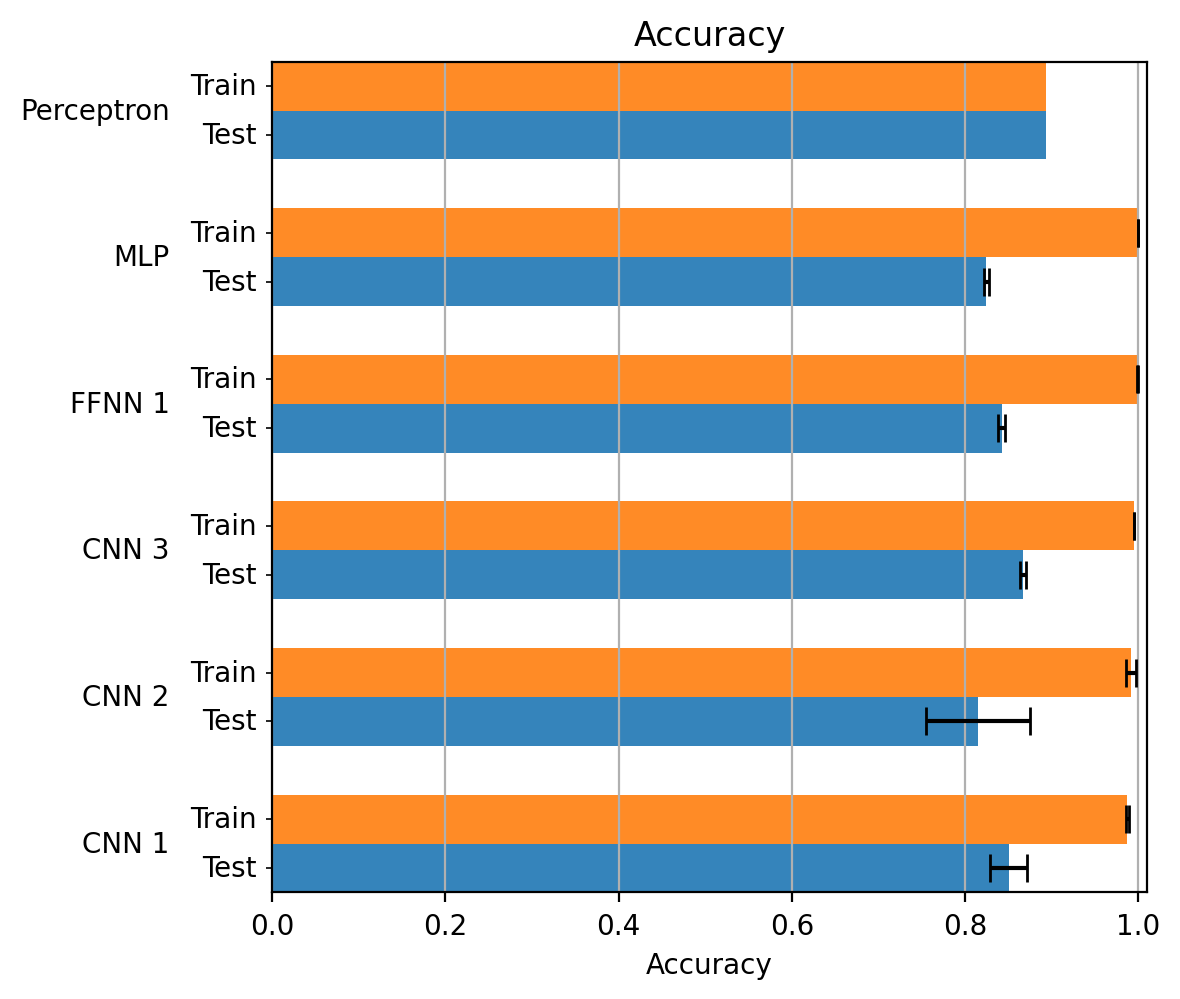
\includegraphics[width=0.82\linewidth]{../images/sequence_results/enhancers/accuracy.png}
\caption{Accuracy metric for enhancers sequence experiments}
\end{figure}
\newpage
\textbf{AUROC}

\begin{longtable}[]{@{}lll@{}}
\toprule
\textbf{Models} & \textbf{Training} & \textbf{Test}\tabularnewline
\midrule
\endhead
Perceptron & mean = 0.5865 & mean = 0.5017\tabularnewline
& STD = 0.0012 & STD = 0.0032\tabularnewline
MLP & mean = 1.0 & mean = 0.4973\tabularnewline
& STD = 0.0 & STD = 0.0047\tabularnewline
FFNN\_1 & mean = 0.9999 & mean = 0.4976\tabularnewline
& STD = 0.0 & STD = 0.0026\tabularnewline
CNN\_1 & mean = 0.9969 & mean = 0.5071\tabularnewline
& STD = 0.0006 & STD = 0.0008\tabularnewline
CNN\_2 & mean = 0.9966 & mean = 0.4949\tabularnewline
& STD = 0.0022 & STD = 0.0028\tabularnewline
CNN\_3 & mean = 0.9988 & mean = 0.4976\tabularnewline
& STD = 0.0002 & STD = 0.0023\tabularnewline
\bottomrule
\end{longtable}

\begin{figure}[h!]
\centering
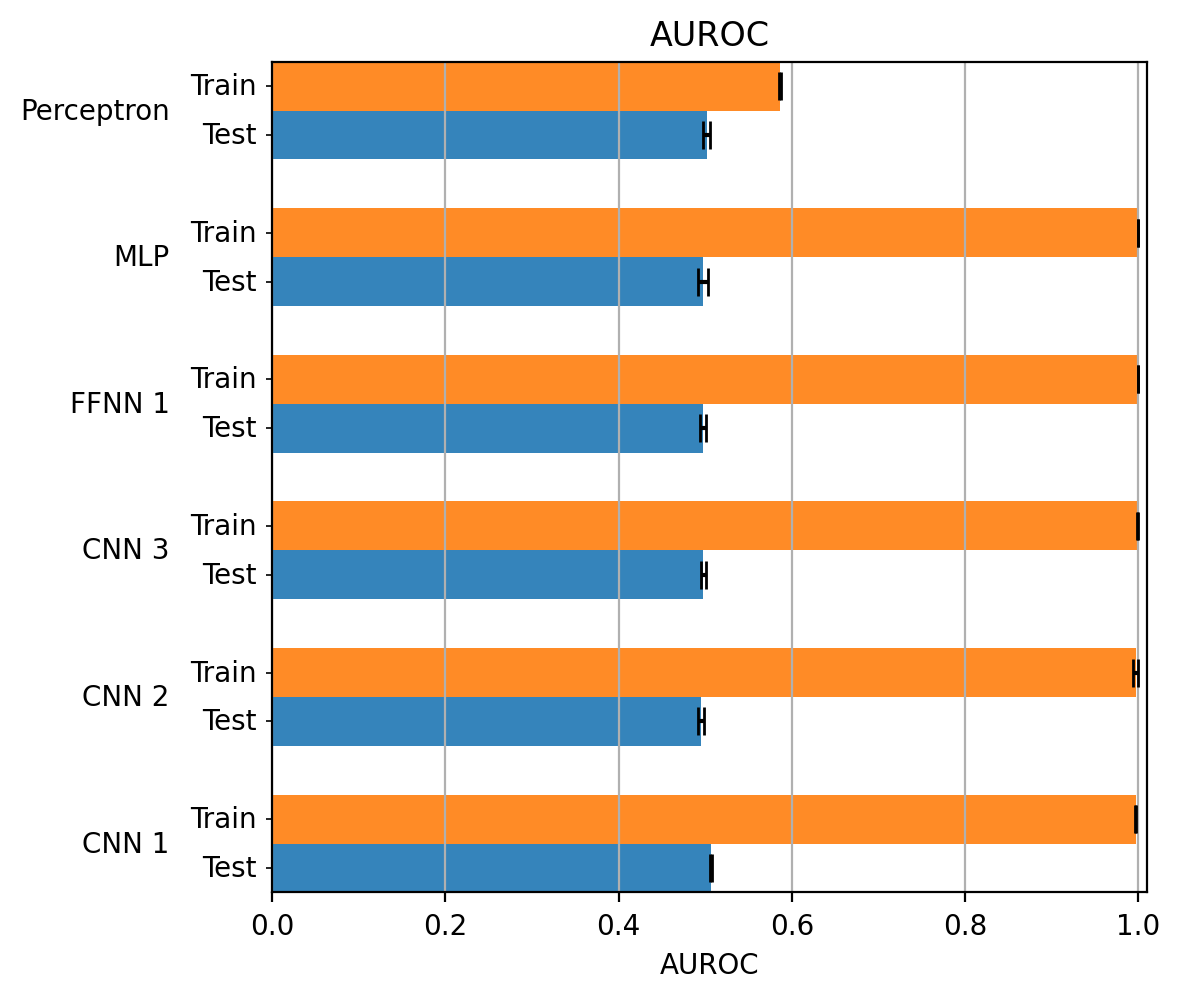
\includegraphics[width=0.8\linewidth]{../images/sequence_results/enhancers/auroc.png}
\caption{AUROC metric for enhancers sequence experiments}
\end{figure}
\newpage
\textbf{AUPRC}

\begin{longtable}[]{@{}lll@{}}
\toprule
\textbf{Models} & \textbf{Training} & \textbf{Test}\tabularnewline
\midrule
\endhead
Perceptron & mean = 0.1413 & mean = 0.1068\tabularnewline
& STD = 0.0013 & STD = 0.0017\tabularnewline
MLP & mean = 1.0 & mean = 0.1046\tabularnewline
& STD = 0.0 & STD = 0.0023\tabularnewline
FFNN\_1 & mean = 0.9997 & mean = 0.1046\tabularnewline
& STD = 0.0002 & STD = 0.0008\tabularnewline
CNN\_1 & mean = 0.9831 & mean = 0.1076\tabularnewline
& STD = 0.0028 & STD = 0.0001\tabularnewline
CNN\_2 & mean = 0.9839 & mean = 0.1041\tabularnewline
& STD = 0.0112 & STD = 0.0015\tabularnewline
CNN\_3 & mean = 0.9906 & mean = 0.1051\tabularnewline
& STD = 0.0015 & STD = 0.0012\tabularnewline
\bottomrule
\end{longtable}

\begin{figure}[h!]
\centering
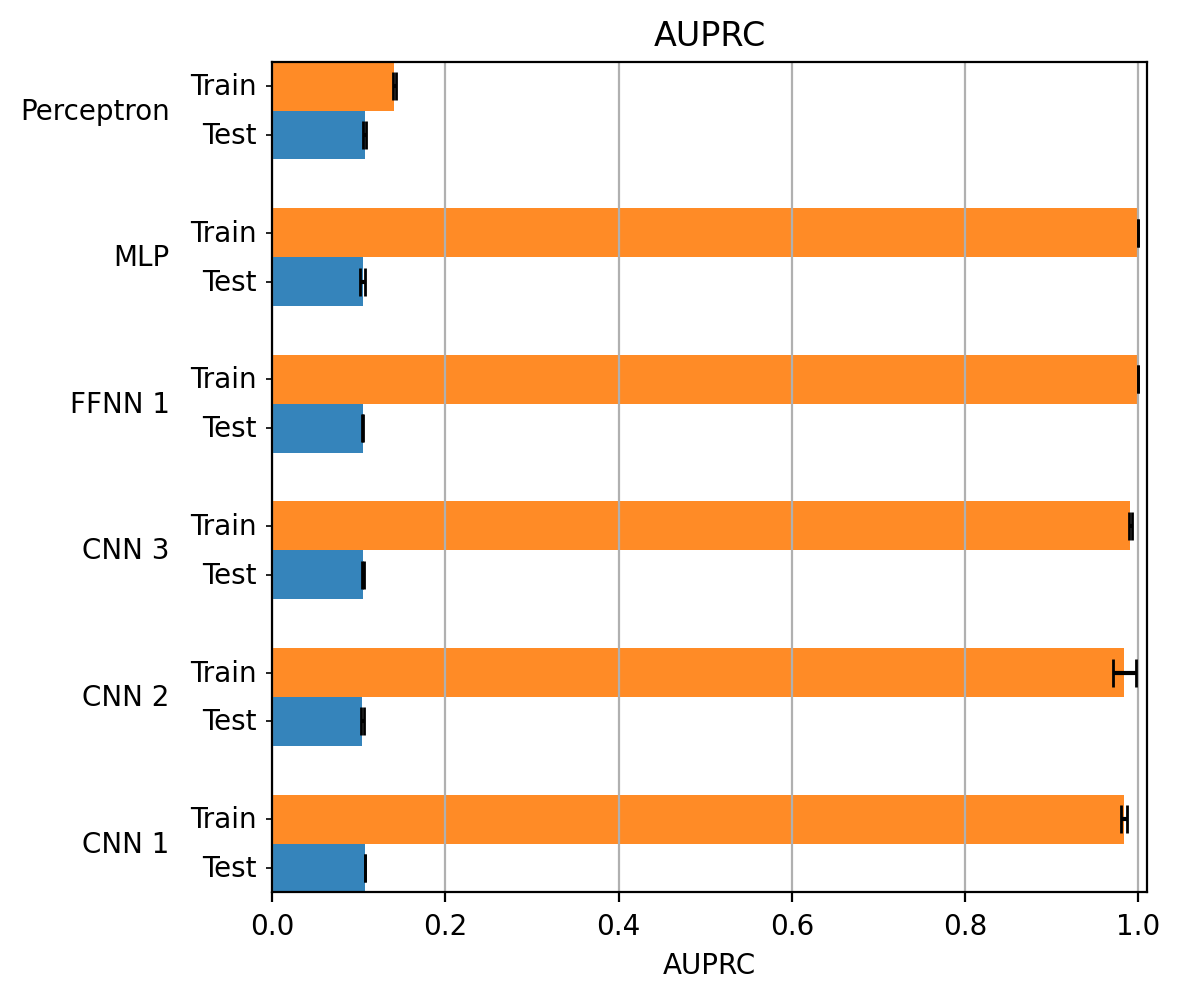
\includegraphics[width=0.8\linewidth]{../images/sequence_results/enhancers/auprc.png}
\caption{AUPRC metric for enhancers sequence experiments}
\end{figure}

\subsubsection{Observations}\label{header-n1829}

\emph{1) The sequence data are insufficient to execute all the tasks.}
The accuracy metrics show that the models have good performances but the
AUPRC and AUROC metrics reveal the opposite, both for promoters and
enhancers. In particular, the AUROC is closed to its minimum values in
all experiments, like the AUPRC. This means that the models return
casual values. These results are confirmed by the data decomposition
graphs, that highlight a total data inseparability. The CNNs, which
should learn automatically the hidden features of the data, can't
improve the performances. The Wilcoxon test shows that the models are statistically identical.

\emph{2) The overfitting problem has not been resolved.} The AUPRC and
AUROC metrics show that the models are not able to generalize and the
high value of accuracy is caused by the data imbalance.

\section{Conclusions}

Using the HEK293 cell line, the experiments results, validated with the
Wilcoxon tests, shows that the feed-forward neural networks can
predict the active and inactive regulatory region using epigenomic data more accurately than the other models using the epigenomic data. However, given the data
complexity, this is true if the networks prevent the overfitting,
otherwise the models aren't able to generalize. This is confirmed by the
perceptron's results, which works similarly to more complex networks.
Despite this, observing the ARPC, it is clear that the task remains difficult. This metric is low compared to the others and it means a low AUPRC means that the models fail to recognize the positive samples. 
For enhancers this fact is particularly pronounced.
In general, the experiments on the epigenomic data show that on HEK293 cell line the deep networks perform well only if their architecture is extremely simple (as in the case of the perceptron). For more complex models it is necessary to adopt aggressive techniques to prevent overfitting.
Instead using the sequence data, the tasks to determine active and
inactive regulatory region do not obtain good results. The models,
including the CNNs, aren't able to learn the complex distribution of
data. These results are confirmed by the data decomposition graphs, which show the total overlap of the active and inactive regulatory region sequence data.